\section{The \lhcb software }
\label{sec:lhcb:soft}

\subsection{The LHCb software}

The processing of the data from the detector in \lhcb is controlled by custom software applications~\cite{Corti:2006yx}.
Each of these software applications is based on the \gaudi framework~\cite{Antunes-Nobrega:630827} 
which provides libraries and a custom API written in \cpp and \python to integrate the common requirements and features needed in
 particle physics software.
The organisation of the \lhcb software for data analyses can be separated into three different components.
First, the trigger software (\moore) runs the \hlt and processes the detector output.
Then, the reconstruction software (\brunel) performs a complete event reconstruction of events that pass the trigger.
This takes into account the understanding of the detector and the conditions under which the detector was run.
Finally, the analysis software (\davinci) runs algorithms that process the fully reconstructed event.
%This allows for further selection of specific types of events containing physics of interest and higher level  processing of the data.

\subsection{Simulation of the \lhcb data}

Simulated data is a large part of data analysis due to the rarity of many \bquark-hadron decays of interest.
There are two applications that are unique to the simulation of events in \lhcb, one to simulate the physics and one to simulate the 
detector hardware~\cite{LHCb-PROC-2011-006}.
The physics simulation application, \gauss, contains several different stand-alone programs.
The underlying event from the $pp$ collision is simulated using \pythia~\cite{Sjostrand:2006za,LHCb-PROC-2010-056}.
Signal decays, for example \BdToKstmm, are generated specifically using \evtgen~\cite{Lange:2001uf}.
The simulated particles coming from \pythia are also processed with \evtgen to determine at what state they enter the detector.
The interactions of the particles with the detector are simulated using \geant~\cite{Agostinelli:2002hh,Allison:2006ve}.
The response of the \lhcb detector hardware to the simulated particles is simulated using \boole, which both digitises the simulated event data
and writes the simulation into a format equivalent to the output of the detector hardware.

There are three different simulations of the \lhcb detector used in Chapters~\ref{chap:kstmm} and~\ref{chap:swave:meas}. 
Each of them corresponds to the best simulation conditions known in 2009, 2010 and 2011 and are called MC09, MC10 and MC11 respectively.
The first of these, MC09 corresponds to the best estimate of the detector performance before the running of the \lhc and the start of data-taking.
This was only used in Section~\ref{sec:lhcb:trigdev} for work performed at the end of 2010.
The second of these simulation configurations, MC10,
contains significant improvements applied as a result of information from the 2010 period of data-taking.
These come from adjustments made to the trigger, the reconstruction and the analysis software along with improvements to the underlying simulation.
The final simulation configuration, MC11, was defined after the end of data-taking in 
2011 and uses the best information available at that point in time.
The analyses of \BdToKstmm presented in Chapter~\ref{chap:kstmm} use both MC10 and MC11 simulation based on what was available at the time.

\subsection{Data-simulation agreement}
\label{sec:kstmm:data:mccorr}

%\begin{itemize}
%\item \dots
%\item I suggest here to add a subsection that describes the quality of the simulation. You can say that the general agreement is very good and then mention the three problem areas (occupancy, IP and PID) and how they in turn are dealt with).
%\item 
%\end{itemize}

The agreement between the data and the \lhcb simulation is generally very good  
but there are several significant differences which are the IP resolution, the particle identification for hadrons and the occupancy of the detector. 
There are also minor effects for which the disagreement is smaller, including 
the relative tracking efficiency and the particle identification for muons.
These known differences are corrected for using a variety of methods depending on the type of correction.
The IP resolution is corrected within the simulation itself, whereas the particle identification for hadrons is corrected after 
the events are simulated.
The difference in event occupancy, tracking efficiency, trigger efficiency and the muon identification are
corrected for by applying weights to each simulated event. 


%The resolution of the impact parameter is different between the data and the simulation. 
The IP resolution for pions from data and from MC10 simulation as a function of inverse \pt are shown in Fig.~\ref{fig:ipxres}.
\begin{figure}[tbp]
\centering
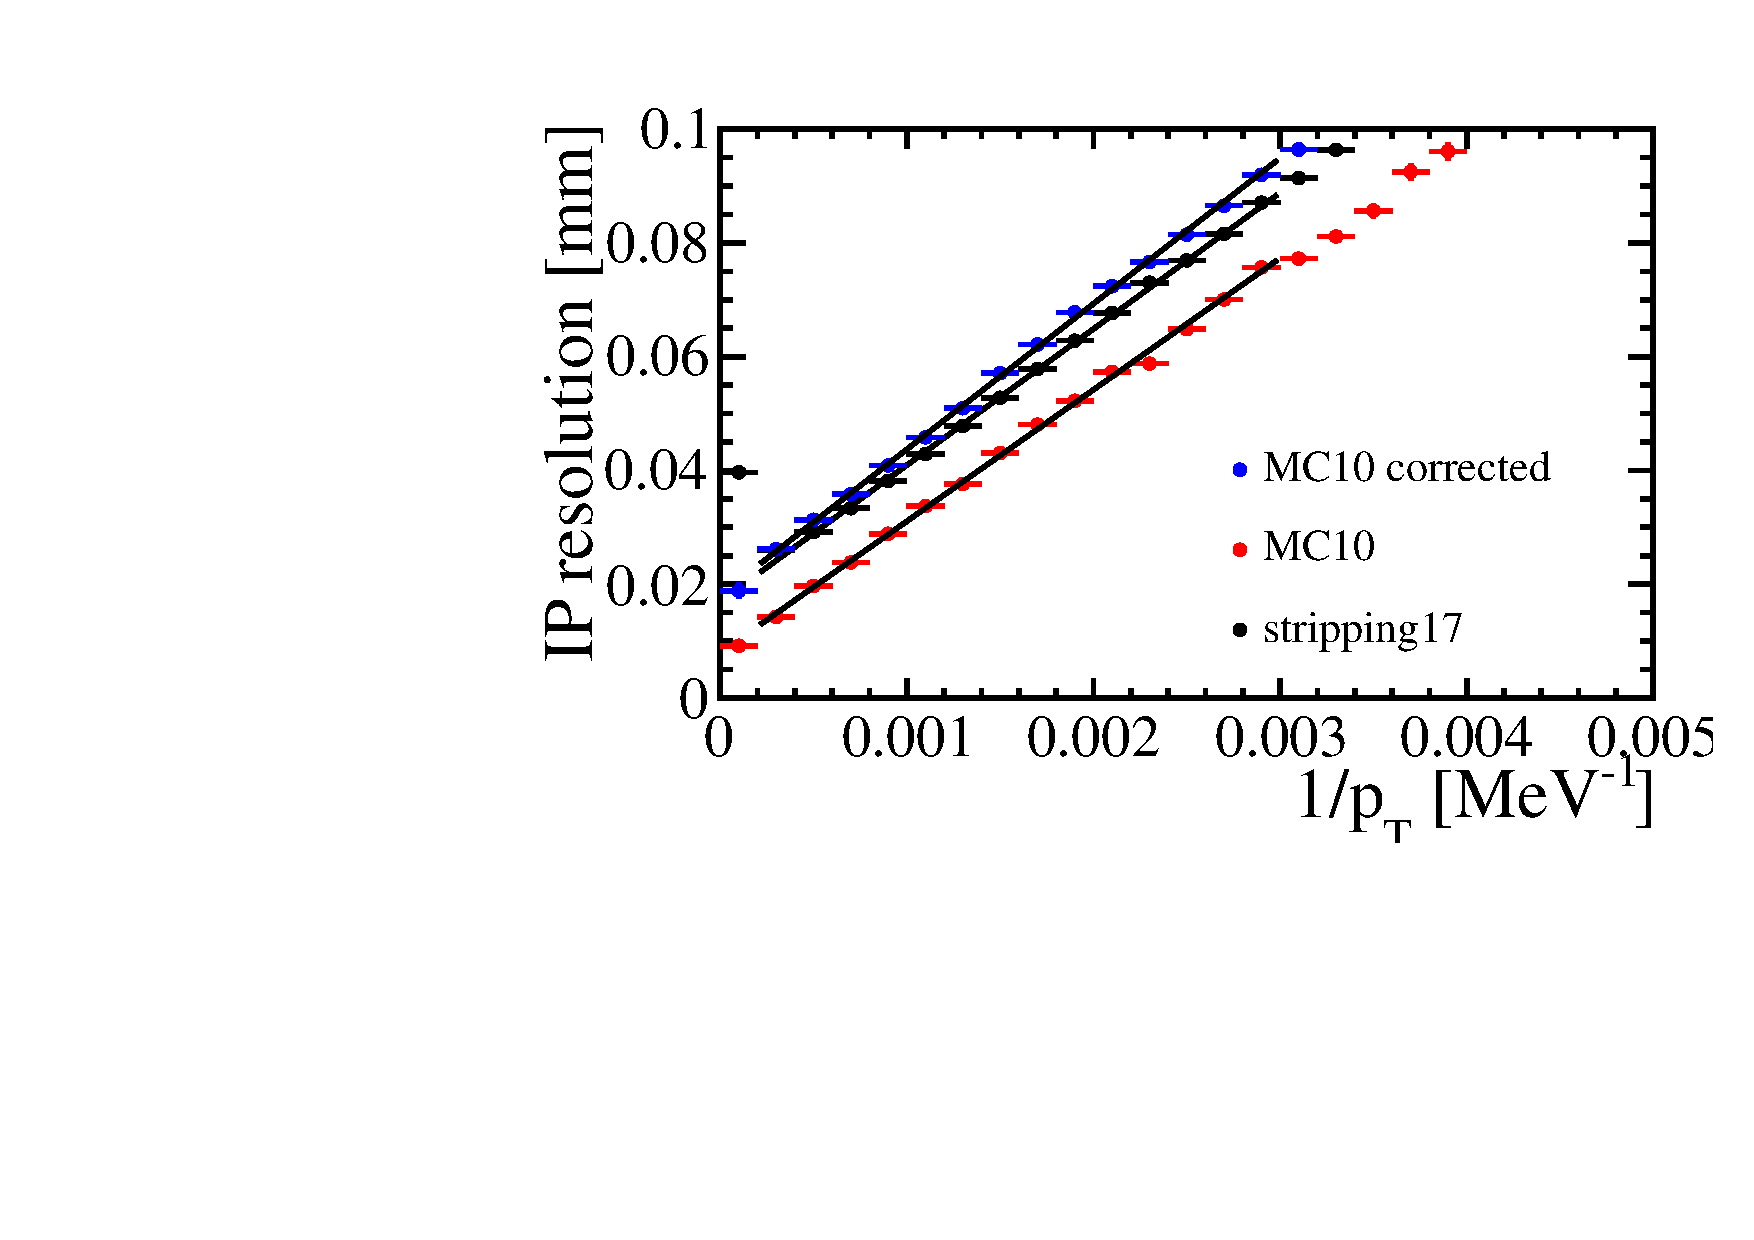
\includegraphics[width=0.48\columnwidth]{chapter5/figs/datamc/ipres_data_mc10_mc10smeared.pdf}
\caption[IP resolution.]{The resolution of the IP in $x$ as a function of inverse \pt for pions from data and simulation. 
The data, labelled `stripping17', is processed with two reconstruction versions used in 2011 and the two simulation
versions are MC10 and MC11. ~\label{fig:ipxres} }
\end{figure}
It is possible to see that the IP resolution is consistently different for both versions of the simulation.
This effect comes from the way the scattering of particles within the material, both in the RF foils and the gas inside the \velo, is simulated.
Contributing factors include the exact description of the amount of material in the \velo in terms of the shape of the RF foils, the alignment of the \velo and the position of the simulated primary vertex.


The IP resolution as a function of $x$ or $y$ for tracks from the primary vertex can be parametrised using a linear function 
\begin{align}
f^{}_{(x/y)\mathrm{data}}(1/\pt) &= a_{(x/y)}\ (1/\pt)  + b_{(x/y)}  \, ,
\end{align}
where $a$ and $b$ are coefficients found for the IP resolution in $x$ and $y$.
The tracks in the simulation can be corrected by smearing the reconstructed track.
%using the difference in the linear functions for data and simulation.
The smearing function is a Gaussian with a zero mean and with the width defined by the difference of the IP resolution for the data and the simulation,
\begin{align}
\sigma_{diff}^{(x/y)} &= \sqrt{ f^{2}_{(x/y),\mathrm{data}}(1/\pt)\, - \, f^{2}_{(x/y),\mathrm{sim}}(1/\pt) } \,  . 
\end{align}
The smeared track is subsequently processed by the reconstruction software which recalculates the new momentum vector for the track. 
%The IP resolution in $x$ for data, corrected and uncorrected pions are shown in Fig.~\ref{fig:ipxcorr}
%\begin{figure}[tbp]
%\caption[Corrected IP resolution.]{The IP resolution in $x$ as a function of inverse \pt for pions from the data, the simulation and the corrected simulation.
%~\label{fig:ipxcorr} }
%\end{figure}

Another significant difference between the data and the simulation is 
the \dll value returned from the pattern recognition in the \rich detectors. 
The difference here is an artifact of the lower 
average occupancy of each simulated event than an average data event.
This is because the higher number of tracks produces more Cherenkov radiation 
which is related to the overall saturation of the HPDs and subsequently the ability for the reconstruction software to match Cherenkov rings to tracks.
The \DLL value for each simulated track was obtained from a sample of 
high purity \Dstarp\to\Dz\pip (and charge conjugate) decays, where the \Dz can be tagged 
using the \pip from the \Dstarp. 
This allows a clean sample of kaons and pions to be selected.
The distribution of the \dllkpi for kaons and pions from \BdToJpsiKstar events before and after the correction was applied 
is shown in Fig.~\ref{fig:dllcomp}.
\begin{figure}[tbp]
\centering
\subfigure{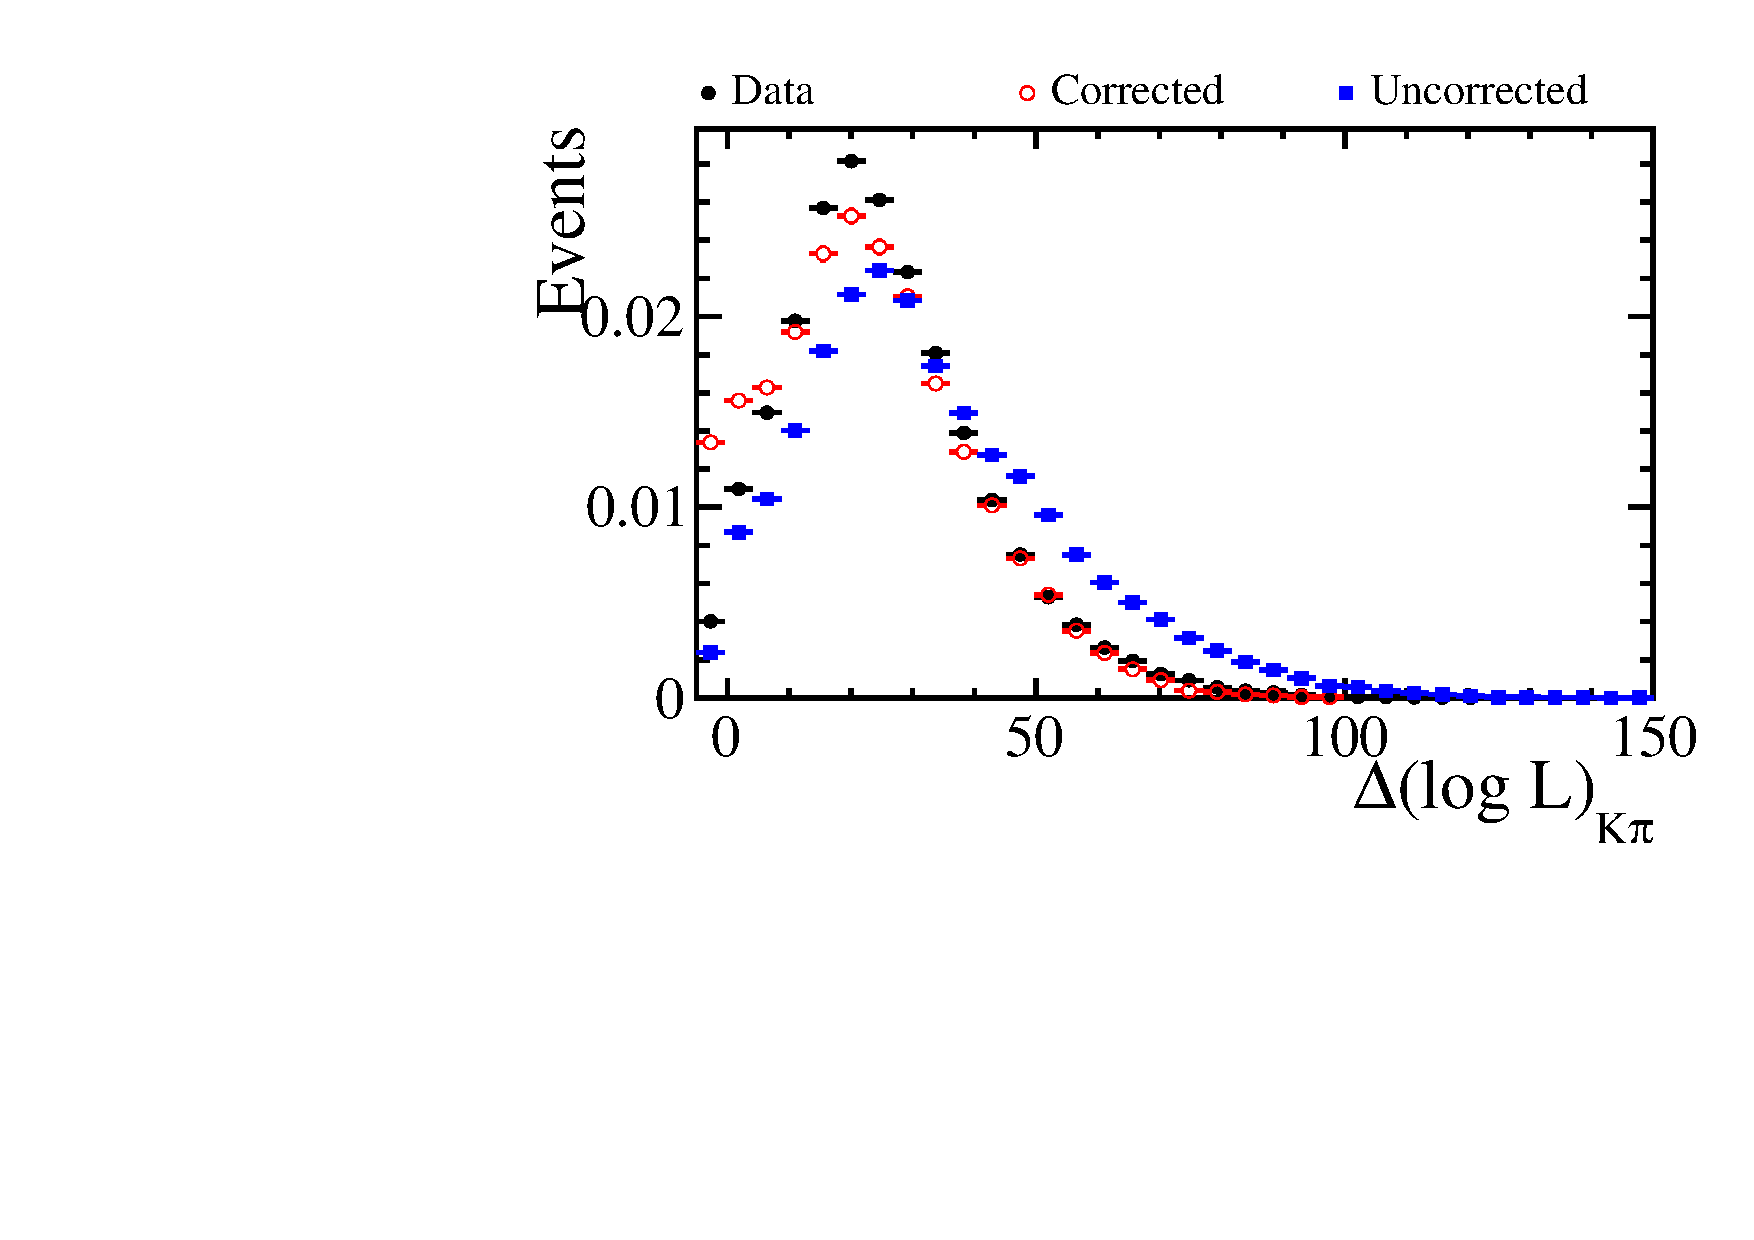
\includegraphics[width=0.48\columnwidth]{appendix/figs/comp_jpsikstar_K_DLLK.pdf}}
\subfigure{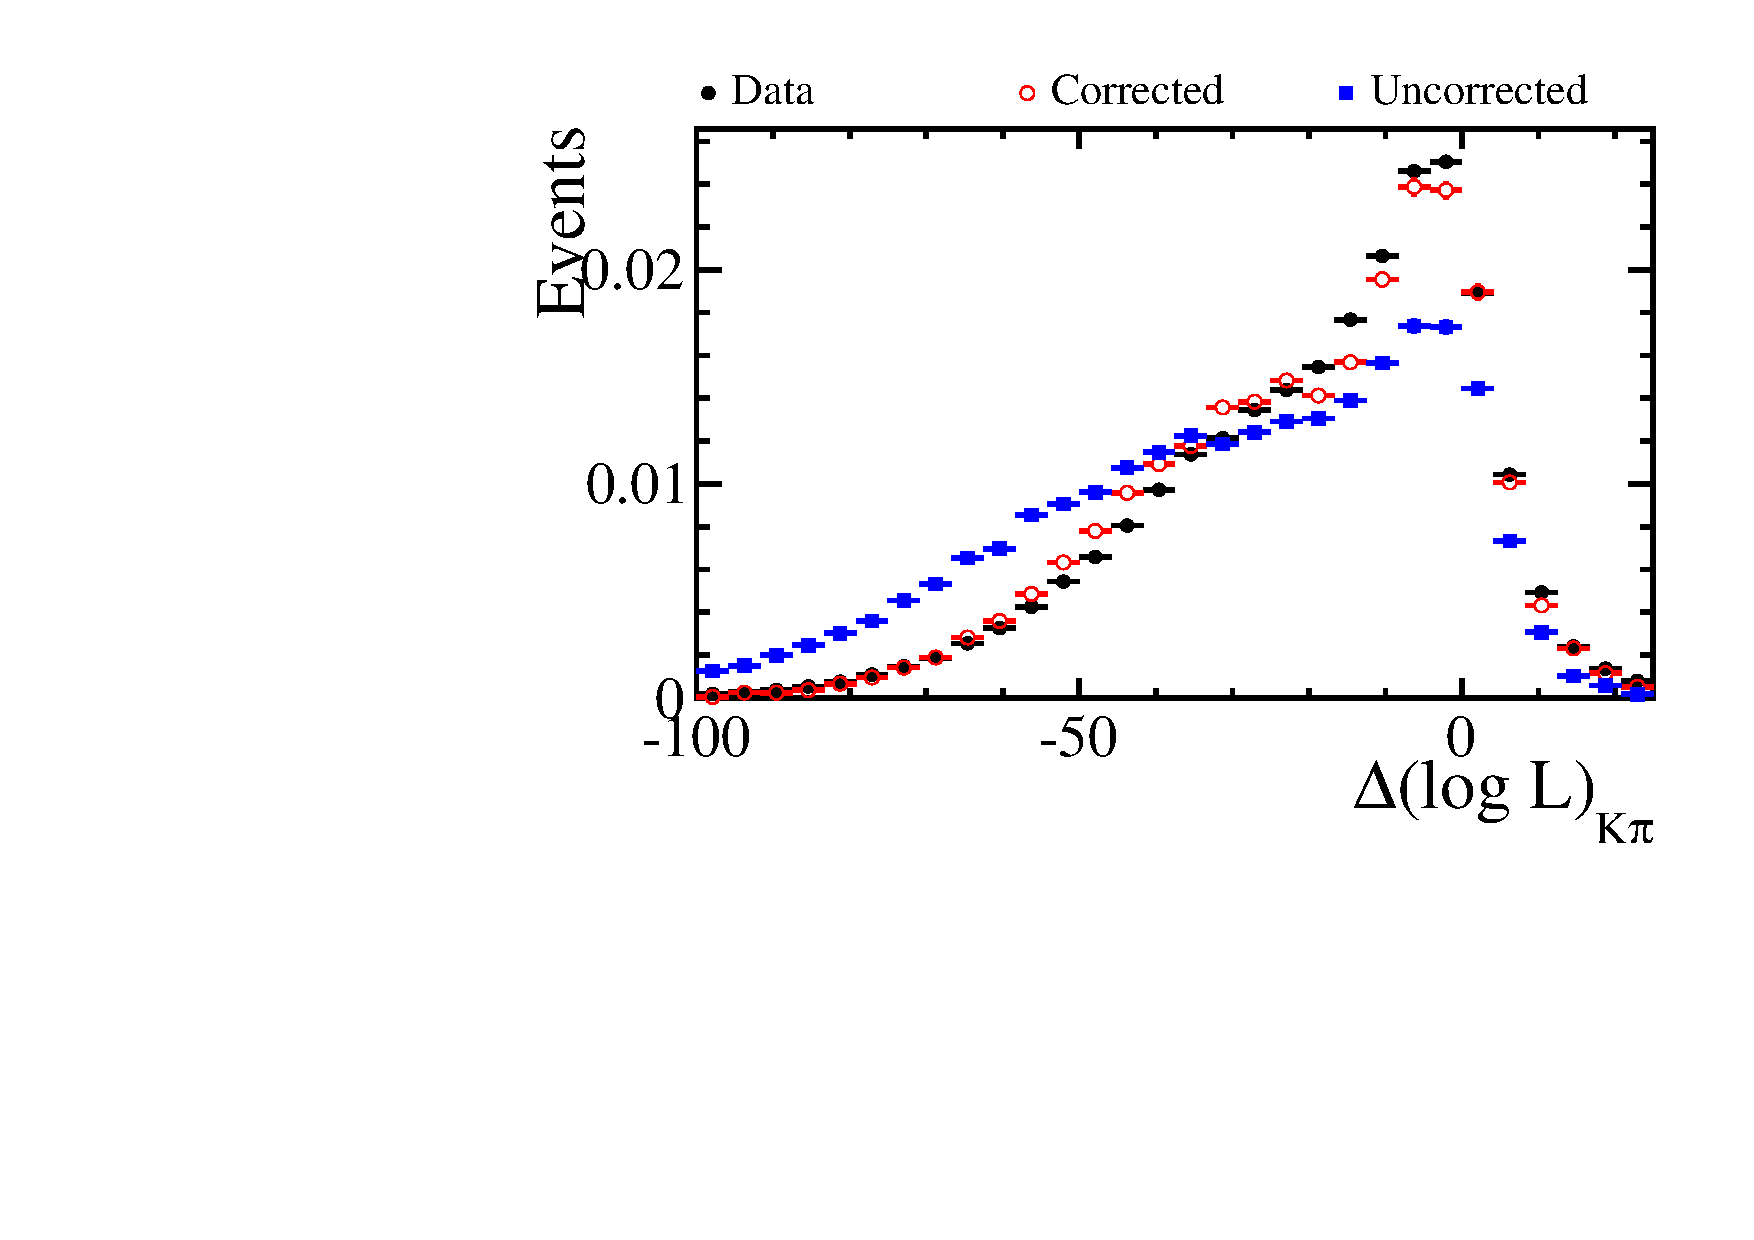
\includegraphics[width=0.48\columnwidth]{appendix/figs/comp_jpsikstar_Pi_DLLK.pdf}}
\caption[Distributions of \dllkpi for pions and kaons.]
{The $\dllkpi$ distributions for (a) kaons and (b) pions to illustrate the difference between data and simulation.
The \BdToJpsiKstar data is shown in black, the uncorrected \BdToJpsiKstar simulation in \textcolor{blue}{blue} and
 the corrected simulation in \textcolor{red}{red}.~\label{fig:dllcomp}}
\end{figure}
It can be seen that there is a significant difference between the \dll distributions for data and uncorrected simulation but that 
there is significantly better agreement after correction.

The third major difference between the data and the simulation is in the overall event occupancy, defined by the number of tracks passing through the detector per event. 
This comes from both the generators used to simulate the proton interaction and also from the description of 
the material in the detector in the simulation.
The simulation is corrected by re-weighting the simulation by the relative difference between data and simulation 
in terms of the number of tracks per event. The ratio between data and simulation is given in Fig.~\ref{fig:trackocc}.
\begin{figure}[tbp]
\centering
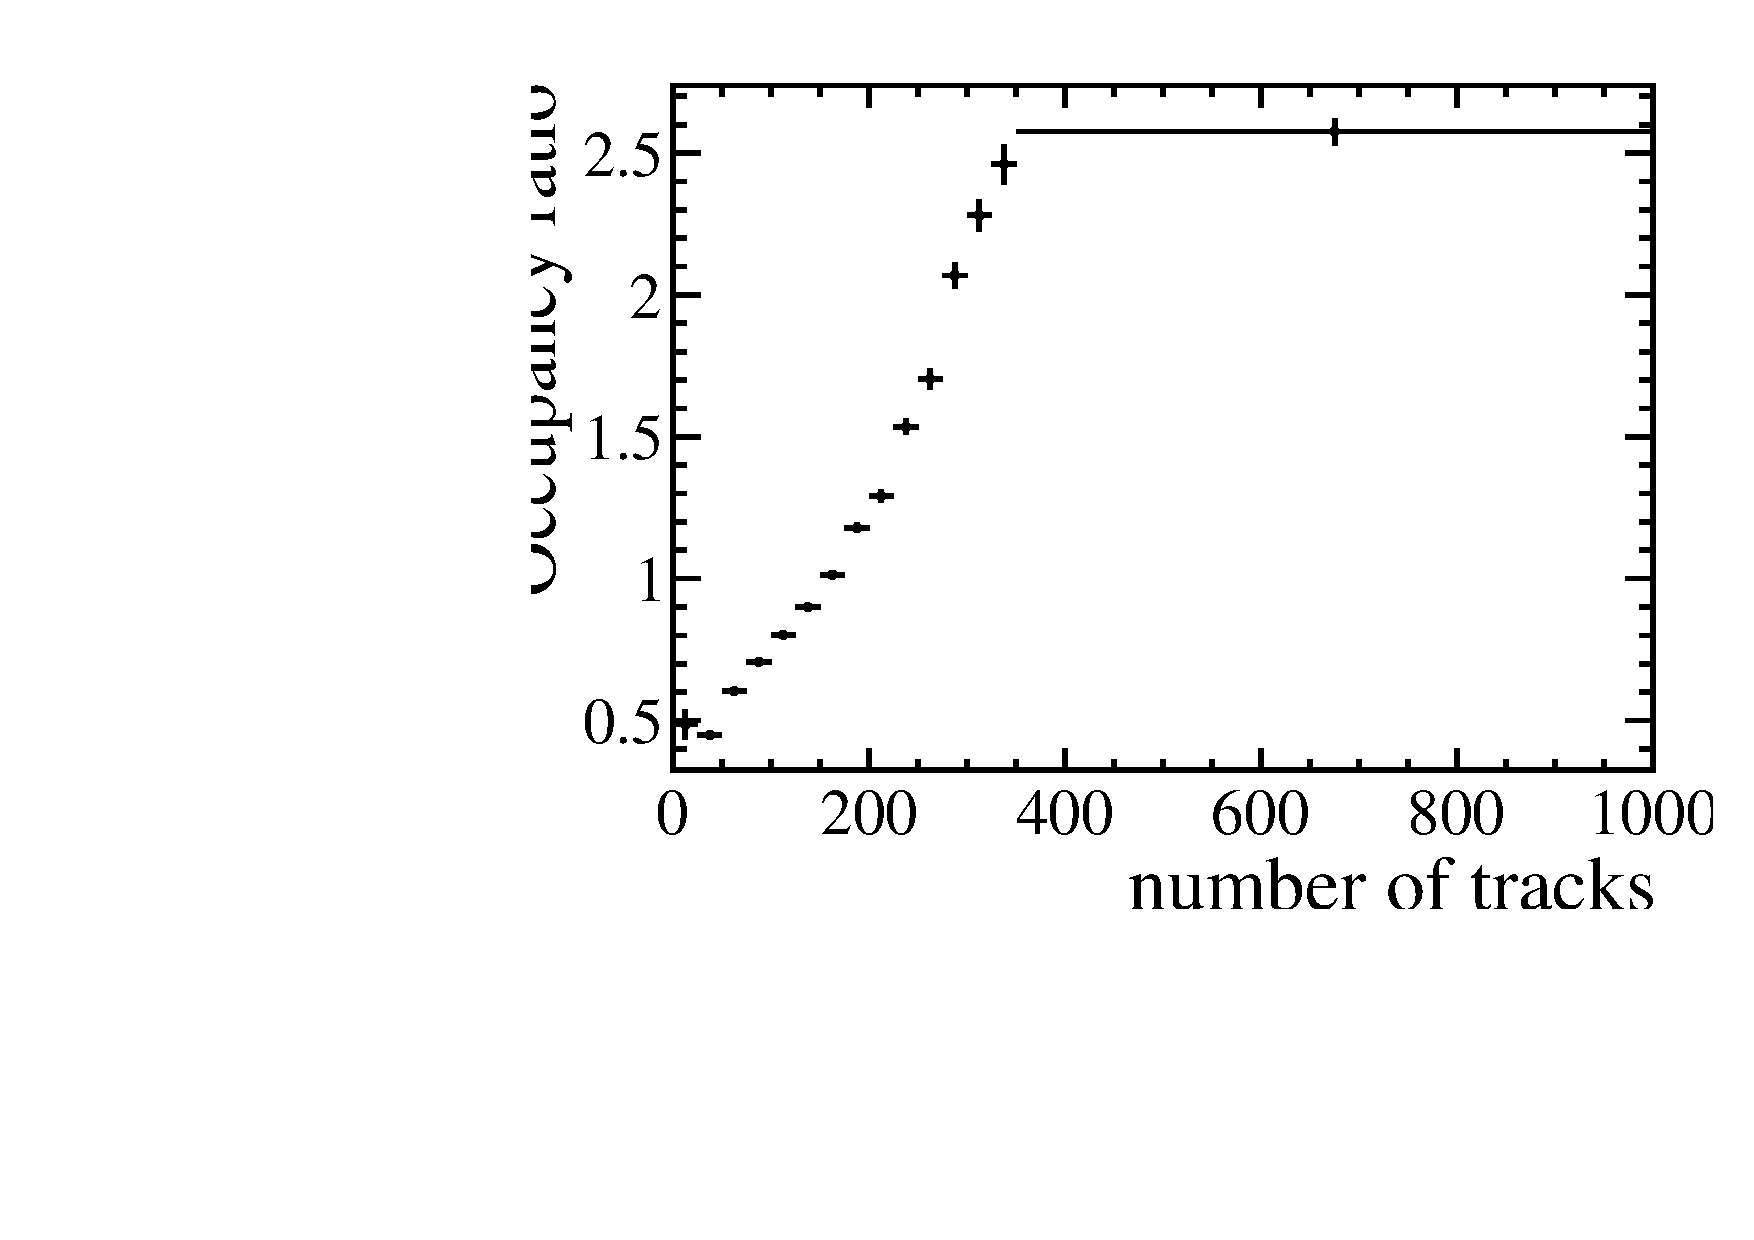
\includegraphics[width=0.48\columnwidth]{chapter5/figs/datamc/track_occ.pdf}
\caption[Event occupancy in data and simulation.]{The relative event occupancy measured by the number of tracks per event
 for selected \BdToJpsiKstar events from data and simulation. 
The data is from the 1.0\invfb sample and the simulation is from MC11.~\label{fig:trackocc}}
\end{figure}
The data/simulation ratio is binned per 25 tracks below 400 tracks and in one single bin above 400 tracks.
This is because there is not enough simulation with an occupancy of above 400 tracks to accurately correct the simulation on a finer level.

The efficiency of muon identification in the data and the simulation is determined by selecting a good sample of muons from \jpsi\to\mumu events using the `tag-and-probe' method.
There are two muon identification parameters considered.
Firstly \verb=IsMuon=, which comes from the muon stations and the relative efficiency for the muon identification flag is shown in Fig.~\ref{fig:ismuon}.
\begin{figure}[tbp]
\centering
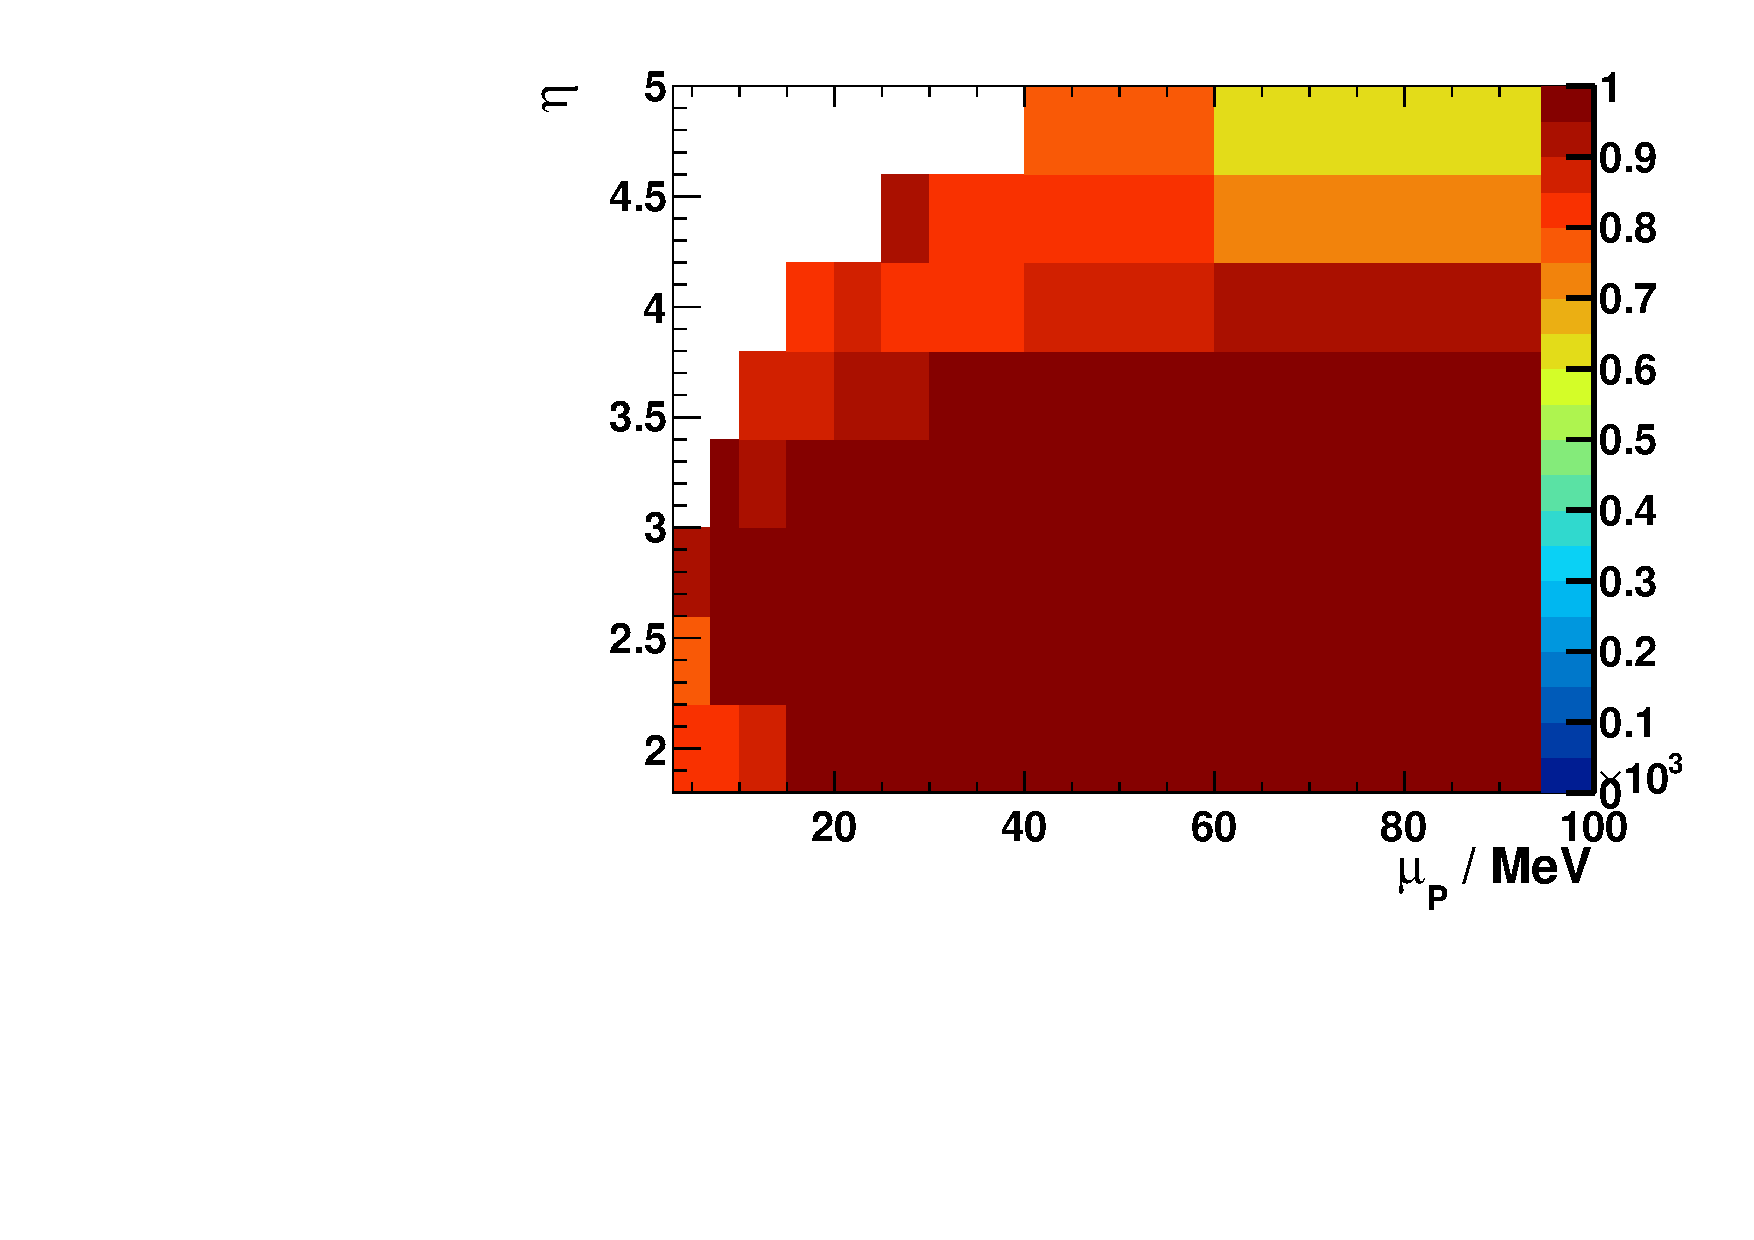
\includegraphics[width=0.48\columnwidth]{chapter5/figs/datamc/isMuon.pdf}
\caption[Muon identification efficiency.]
{The relative muon identification efficiency between data and simulation 
for muons from \jpsi\to\mumu events identified using the `tag-and probe' method~\cite{AlvesJr:1492807}.
The data is from the 1.0\invfb sample and the simulation is MC11.  ~\label{fig:ismuon}}
\end{figure}
It can be seen that there is good agreement between the data and simulation for the muon identification flag.
The relatively uniform values for the relative efficiency allows each data event to be weighted based on the relative efficiency as a function of the momentum of both muons.
The \DLL value for muons is obtained from the data in a similar way to the hadron particle identification but using selected muons from the \jpsi\to\mumu sample.

The relative tracking efficiency for all tracks in the \lhcb detector 
can be determined using the `tag-and-probe' method on pions from a high purity sample of reconstructed \KS\to\pipi candidates.
The relative efficiency between data and simulation can be seen in Fig.~\ref{fig:trackeff}.
\begin{figure}[tbp]
\centering
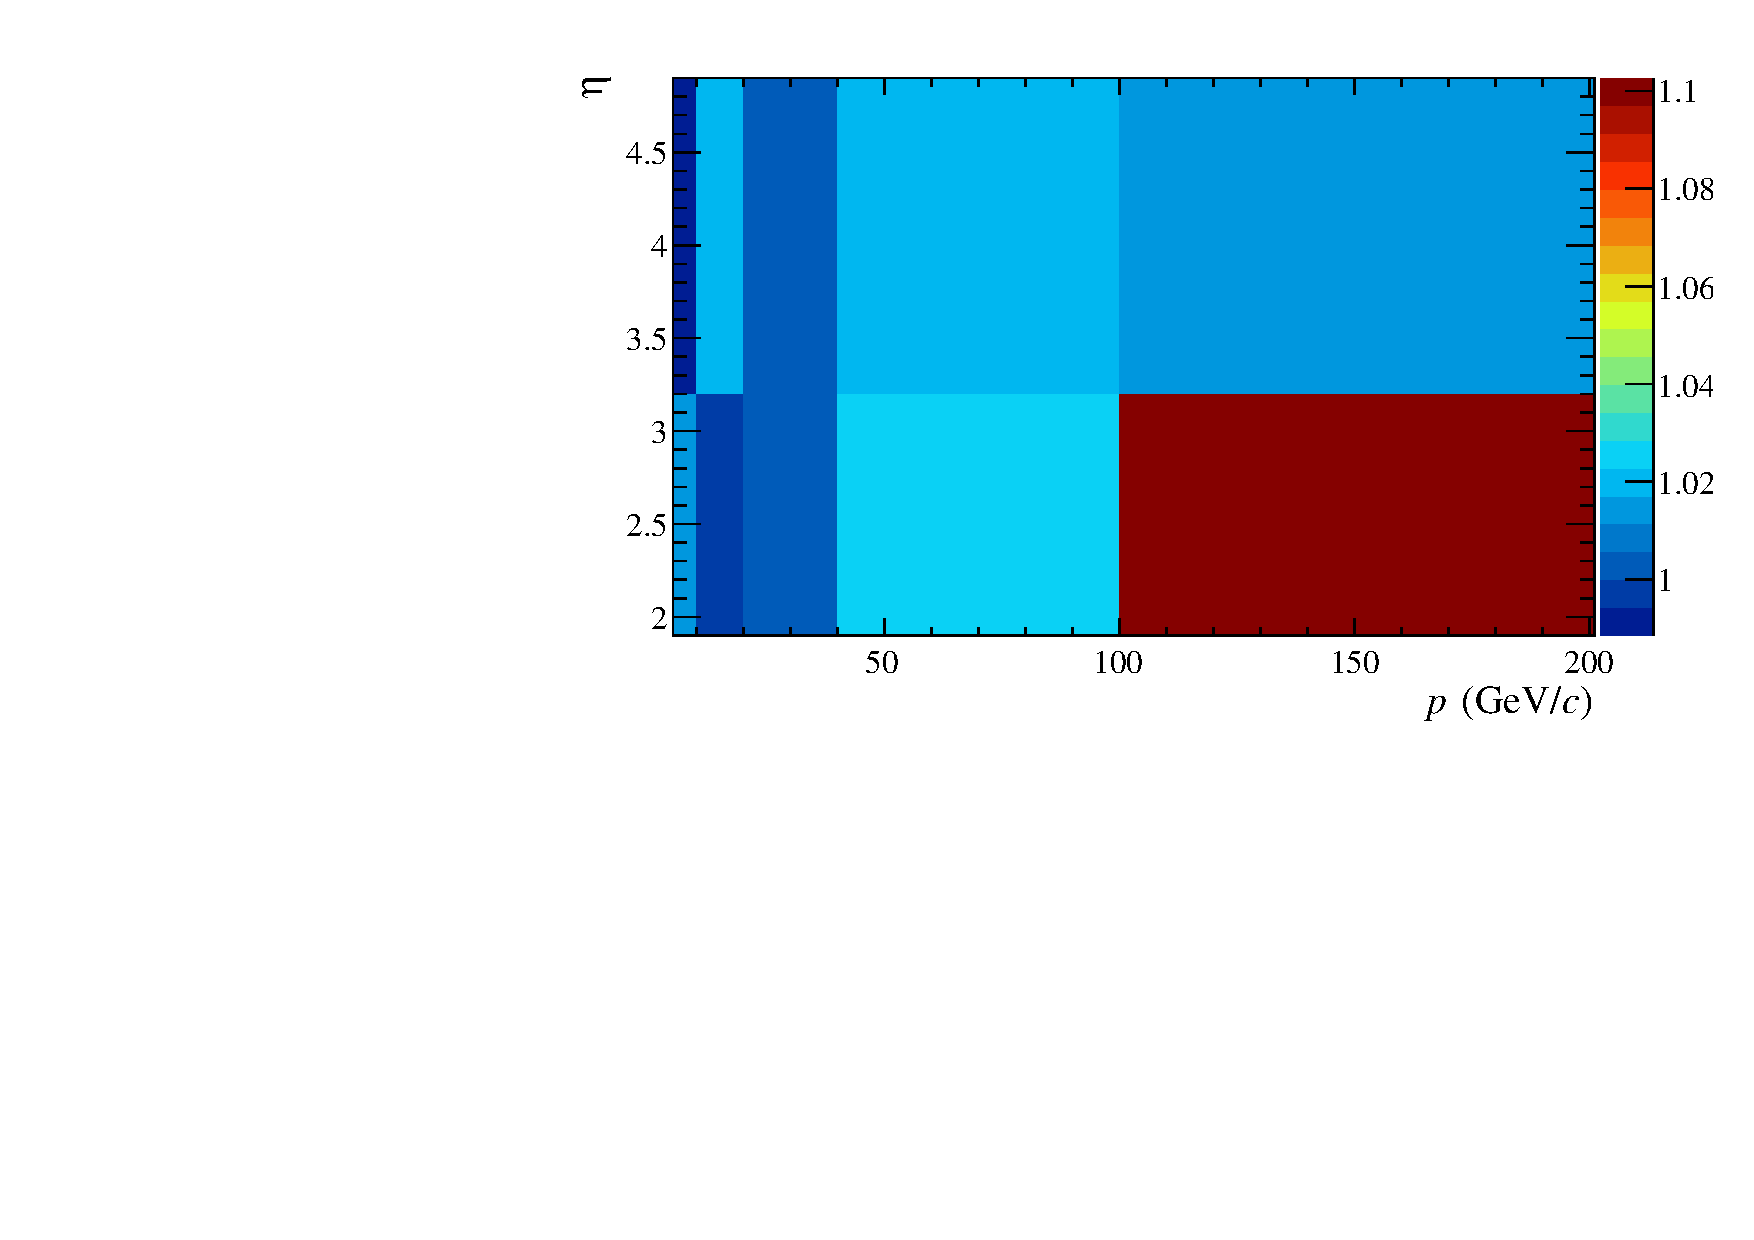
\includegraphics[width=0.48\columnwidth]{chapter5/figs/datamc/track_eff_ratio.pdf}
\caption[Tracking efficiency for data and simulation.]
{The ratio of tracking efficiency between data and simulation for pions from \KS\to\pipi 
decays selected from the 1.0\invfb data and MC11 simulated events~\cite{LHCb-PUB-2011-025}.~\label{fig:trackeff}}
\end{figure}
The simulated events are weighted by the relative efficiency for each of the four tracks in the decay.

After all of the above corrections and weights have been applied, 
there are residual differences between  data and simulation in the momentum spectrum of the \Bd.
The ratio of \Bd momentum between data and simulation for \BdToJpsiKstar events from data and simulation is shown in Fig~\ref{fig:ratiobp}.
\begin{figure}[tbp]
\centering
\subfigure{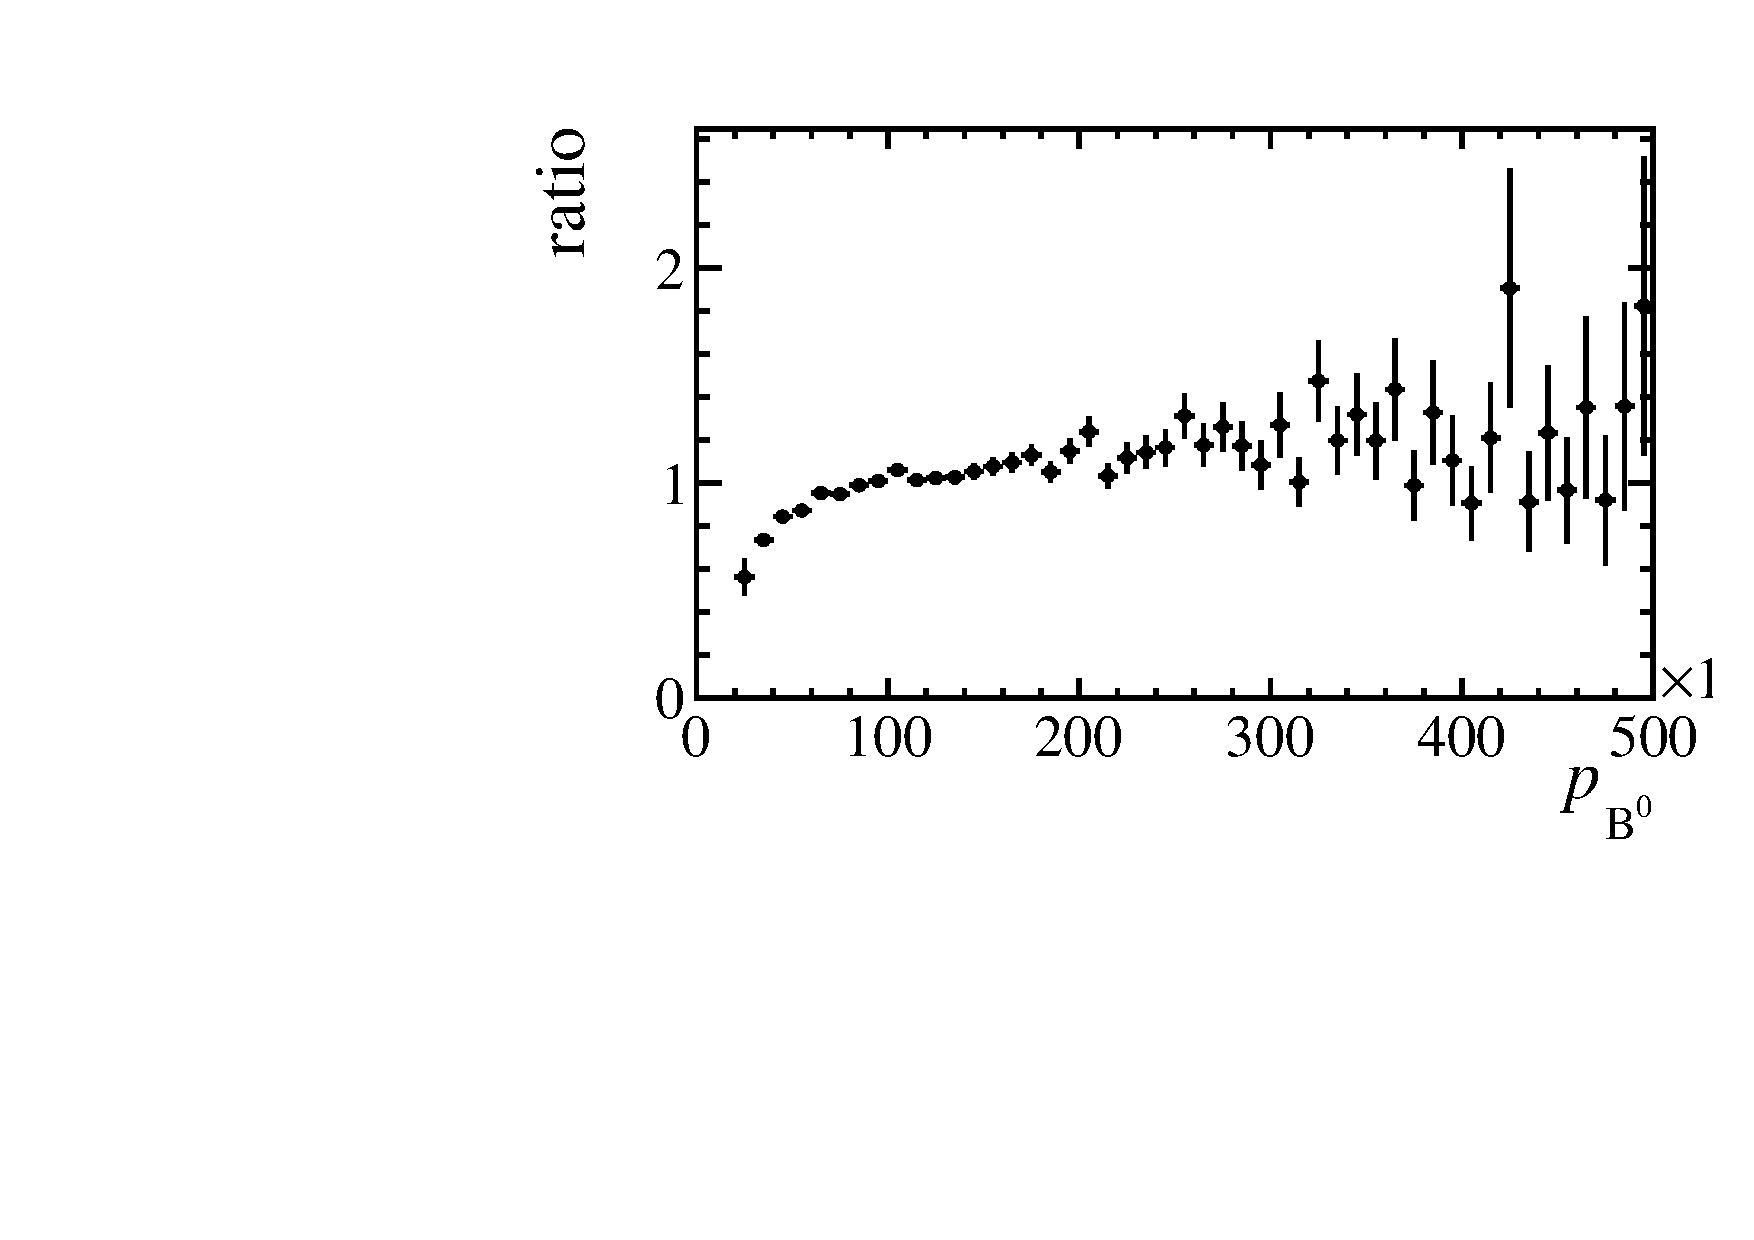
\includegraphics[width=0.48\columnwidth]{appendix/figs/comp_jpsikstar_ratio_B0_P.pdf}}
\caption[The ration between data and simulation of the \Bd momentum distribution]
{The ratio of the \Bd momentum distribution for selected \BdToJpsiKstar events from the 1.0\invfb data sample and from MC11 simulated events.
It is possible to see that the ratio diverges from unity at both low and high momenta. ~\label{fig:ratiobp}}
\end{figure}
The \Bd momentum spectra is corrected by weighting the simulated events by the ratio of data when compared to simulation.
The total weight given to a \BdToKstmm simulated event, for example, is 
\begin{align}
\omega( P_{\mun},P_{\mup},P_{\pion},P_{\kaon},P_{\Bd})   &=  \omega_{\text{IsMuon}}^{\mun}(P_{\mun}) \times \omega_{\text{IsMuon}}^{\mup}(P_{\mup})  \nonumber \\ 
    &  \times  \omega_{trackeff}^{\pion}(P_{\pion}) \times \omega_{trackeff}^{\kaon}(P_{\kaon})  \nonumber \\ 
&   \times \omega_{trackeff}^{\mun}(P_{\mun}) \times \omega_{trackeff}^{\mup}(P_{\mup}) \nonumber \\
    & \times \omega_{P}(P_{\Bd})  \, .
\end{align}
